\documentclass[tikz,border=3pt]{standalone}
\usetikzlibrary{positioning,arrows.meta,shapes.geometric,backgrounds}

\begin{document}

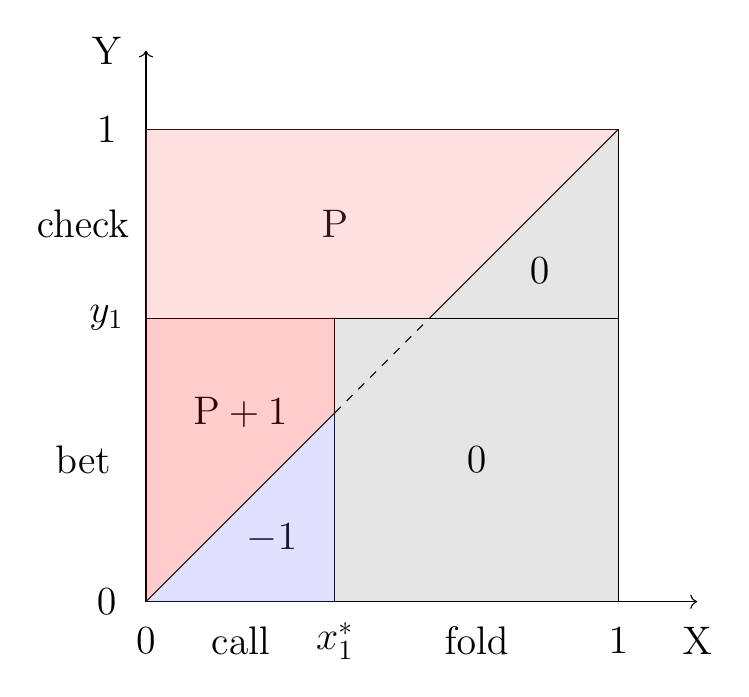
\begin{tikzpicture}

%%% 定型
\draw[->] (0,0) --(0,7);
\draw[->] (0,0) --(7,0);
\draw (0,6) --(6,6) --(6,0);

\node[font=\Large] at (7,-0.5) {X};
\node[font=\Large] at (-0.5,7) {Y};

\node[font=\Large] at (0,-0.5) {$0$};
\node[font=\Large] at (6,-0.5) {$1$};
\node[font=\Large] at (-0.5,0) {$0$};
\node[font=\Large] at (-0.5,6) {$1$};
%%%

%% 線
\draw (0,3.6) --(6,3.6);
\draw (2.4,0) --(2.4,3.6);

\draw (0,0) --(2.4,2.4);
\draw[dashed] (2.4,2.4) --(3.6,3.6);
\draw (3.6,3.6) --(6,6);

%% 目盛り
\node[font=\Large] at (2.4,-0.5) {$x_1^*$};
\node[font=\Large] at (-0.5,3.6) {$y_1$};

%% 数字
\node[font=\Large] at (2.4,4.8) {$\mathrm{P}$};
\node[font=\Large] at (5.0,4.2) {$0$};
\node[font=\Large] at (4.2,1.8) {$0$};
\node[font=\Large] at (1.2,2.4) {$\mathrm{P}+1$};
\node[font=\Large] at (1.6,0.8) {$-1$};

%% 範囲説明
% X axis
\node[font=\Large] at (1.2,-0.5) {call};
\node[font=\Large] at (4.2,-0.5) {fold};
% Y axis
\node[font=\Large] at (-0.8,4.8) {check};
\node[font=\Large] at (-0.8,1.8) {bet};

%% 色
\fill[black, opacity=0.1] (2.4,0) rectangle (6,3.6);
\fill[black, opacity=0.1] (3.6,3.6) --(6,3.6) --(6,6) --cycle;

\fill[blue!60, opacity=0.2] (0,0) --(2.4,0) --(2.4,2.4) --cycle;

\fill[red, opacity=0.2] (0,0) --(2.4,2.4) --(2.4,3.6) --(0,3.6) --cycle;
\fill[red!60, opacity=0.2] (0,3.6) --(3.6,3.6) --(6,6) --(0,6) --cycle;

\end{tikzpicture}
\end{document}
